\documentclass[a4paper,10pt]{article} % Use 10pt font size
\usepackage{graphicx}
\usepackage{fancyhdr}
\usepackage{geometry}
\usepackage{amsmath}
\usepackage{blindtext}
\usepackage{booktabs}
\usepackage{tabu}
\usepackage{eso-pic}
\usepackage{atbegshi}
\usepackage[export]{adjustbox}
\usepackage{float} % For H placement option
\usepackage{caption} % For adjusting caption settings
\usepackage{subcaption} % For subfigures
\usepackage[10pt]{extsizes} % Set font size to 10pt
\usepackage{setspace}
\setstretch{1.0} % Adjust line spacing
\renewcommand{\normalsize}{\fontsize{12pt}{14pt}\selectfont} % Set font size to 10pt
\usepackage{listings}
\lstset{frame=tb,
  language=cpp,
  aboveskip=3mm,
  belowskip=3mm,
  showstringspaces=false,
  columns=flexible,
  basicstyle={\small\ttfamily},
  numbers=left,
  numberstyle=\tiny\color{gray},
  keywordstyle=\color{blue},
  commentstyle=\color{dkgreen},
  stringstyle=\color{mauve},
  breaklines=true,
  breakatwhitespace=true,
  tabsize=3
}
\usepackage[most]{tcolorbox} % For colored boxes
\usepackage{xcolor}

\definecolor{codebgcolor}{RGB}{240, 240, 240}

\setlength{\parskip}{1em}
\setlength{\parindent}{0em}

% Page Geometry
\geometry{a4paper, total={170mm,257mm}, left=20mm, right=20mm, top=30mm, bottom=30mm, headheight=40pt}

% Page Header/Footer Setup
\pagestyle{fancy}
\fancyhf{}
\lhead{
\includegraphics[width=2cm]{CA/iiitb_logo.jpg}} 
\lfoot{International Institute of Information Technology, Bangalore}
\rfoot{Page \thepage}

\begin{document}

\begin{center}
    \huge{\textbf{MIPS Architecture Design}} \\[8pt]
    \large{Course Name: EG 212, Computer Architecture - Processor Design}\\[20pt]
    \large{Shubhranil Basak IMT2023510} \\[5pt]
    \large{Saheem Showkat Reshi IMT2023051} \\[5pt]
    \large{Sayed Naveed IMT2023119} \\[5pt]
\end{center}

\rule{\textwidth}{0.5pt}
\section*{Introduction:}

MIPS (Microprocessor without Interlocked Pipelined Stages) is a family of reduced instruction set computer (RISC) instruction set architectures (ISA) developed by MIPS Computer Systems, now MIPS Technologies, based in the United States.

There are multiple versions of MIPS: including MIPS I, II, III, IV, and V; as well as five releases of MIPS32/64 (for 32- and 64-bit implementations, respectively). The early MIPS architectures were 32-bit; 64-bit versions were developed later. As of April 2017, the current version of MIPS is MIPS32/64 Release 6. MIPS32/64 primarily differs from MIPS I–V by defining the privileged kernel mode System Control Coprocessor in addition to the user mode architecture.

The MIPS architecture has several optional extensions. MIPS-3D which is a simple set of floating-point SIMD instructions dedicated to common 3D tasks, MDMX (MaDMaX) which is a more extensive integer SIMD instruction set using the 64-bit floating-point registers, MIPS16e which adds compression to the instruction stream to make programs take up less room, and MIPS MT, which adds multithreading capability.\cite{WikipediaIAS}



\section*{Processor:}

We are implementing the simulation of the MIPS processor through python. We take the machine code from the MARS simulator as binary text. We give this machine code to the processor by using fileinput module of python.
We have implemented the data and the instruction memory using dictonary class in python. Our assumption is that the text segment of the processor starts from 0 and ends at 1000. Hence, we are capable of execution 250 instructions in the code space. Our data memory starts at 8000 add ends at 10000. The instruction and data memory store bianry strings.
We have made the processor as a class. We have created fetch, decode, execute, memory access, and writeback as methods of this class. We also have created many other methods and global functions in the file while help us in the simulation.
We implement the different cycles of the processor by calling the class methods like fetch, decode etc. in a while loop in the main program. The simulation of the processor ends when the final exit syscall is encountered. We have used a control variable for breaking out of the while loop after the final syscall.
After the simulation is finished and all the outputs of the program are printed, we also show the values stored in the registers that we have used in the simulation.
The pipelined architecture for the MARS processor is depicted below.

\begin{figure}[H] % Use the H placement option
    \centering
    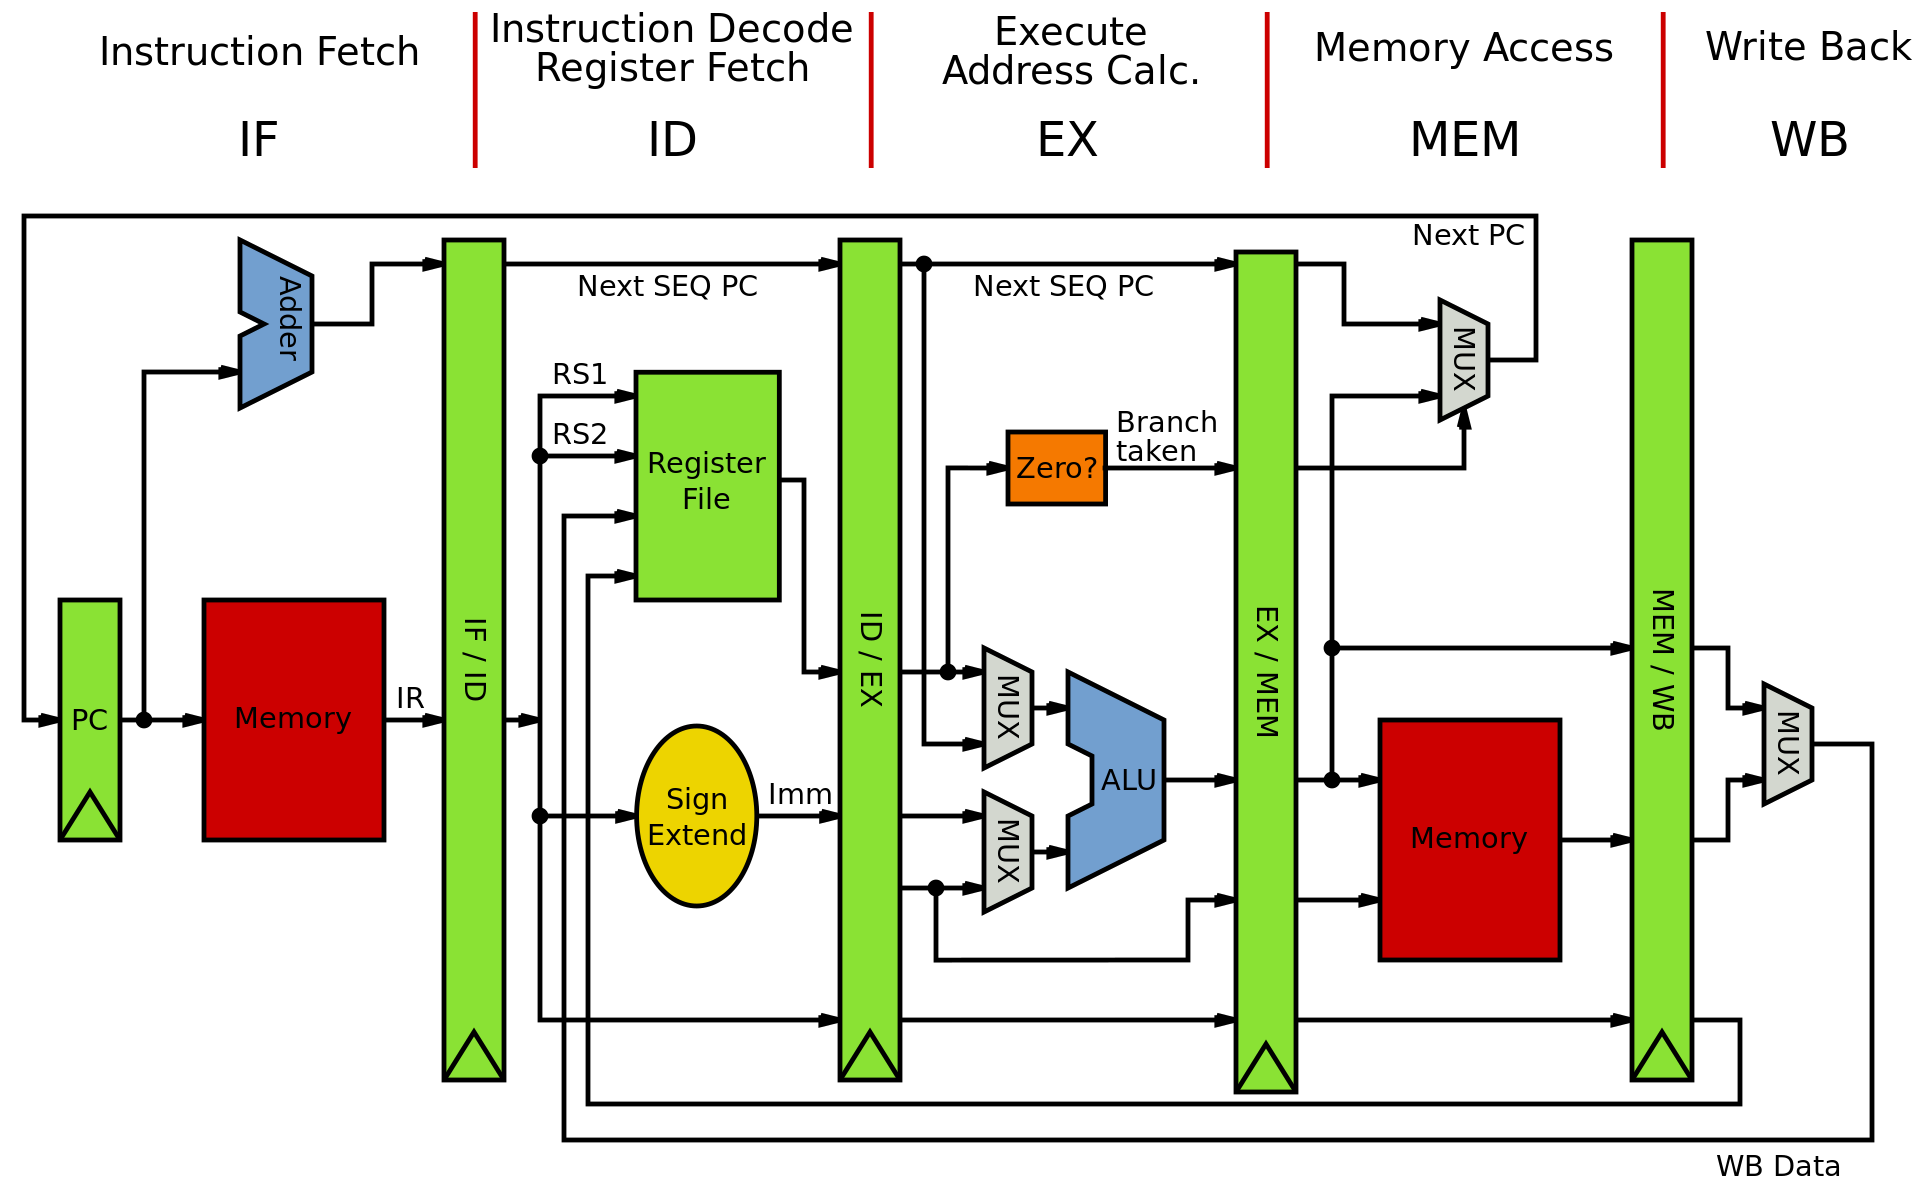
\includegraphics[width=1.0\textwidth]{CA/MIPS_Architecture_(Pipelined).png}
    \caption{MIPS Architecture (Pipelined)}
    \label{fig:IAS Flow Chart}
\end{figure}

\newpage 

\rule{\textwidth}{0.5pt}
\section*{\huge{\textbf{2-Sum Problem:}}}

This program takes a sorted array and also takes a target number, it then returns two numbers from the array that adds up to the target number. In case no such pair exists, the program returns -1.

\subsection*{\Large{Original C++ Code :}}

% Define a new tcolorbox environment for the code

\newtcolorbox{codebox}{
  colback=codebgcolor, % Background color
  colframe=black, % Frame color
  listing only,
  left=0mm,
  right=0mm,
  top=0mm,
  bottom=0mm,
  boxsep=5pt, % Padding around code
  fontupper=\small, % Adjust font size
  enhanced jigsaw
}
\begin{codebox}
    
\begin{lstlisting}[language=C++]
#include<bits/stdc++.h>
using namespace std;
int main(){
    int a[100];
    int size,sum;
    cout<< "Enter the size of the array ";
    cin>>size;
    cout<<"Enter the elements of the array(Each element in a new line)\n";
    for(int i=0;i<size;i++){
        cin>>a[i];
    }
    cout<<"Enter the value of sum ";
    cin>>sum;
    int i=0,j=size-1;
    int flag=0;
    while(i<j){
        if(a[i]+a[j]==sum){
            cout<<a[i]<<" "<<a[j];
            flag=1;
            break;
        }
        else if(a[i]+a[j]<sum){
            i+=1;
        }
        else{
            j-=1;
        }
    }
    if(!flag){
        cout<<-1<<endl;
    }
}
\end{lstlisting} 
\end{codebox}
\newpage

\section*{\huge{\textbf{Assembly Code:}}}

Equivalent to the above C++ code we will write a assembly code in MIPS format.

\subsection*{\large{\textbf{Assembly Code:}}}

\newtcolorbox{codebox}{
  colback=codebgcolor, % Background color
  colframe=black, % Frame color
  listing only,
  left=0mm,
  right=0mm,
  top=0mm,
  bottom=0mm,
  boxsep=2pt, % Padding around code
  enhanced jigsaw % Allow page breaks inside the box
}
\begin{codebox} 
\begin{lstlisting}[language=Assembly]
findsum:
	#s5=i,s6=j
	move $s5,$zero #s5,i=0
	addi $t0,$t0,-1 #size=size-1
	move $s6,$t0 #j=size-1
	move $s3,$zero #flag=0 , s3=flag
	whiles:
		bge $s5,$s6,flag #if i>=j check flag
		mul $t3,$s5,4 	 #t3=s5*4 (i*4)
		mul $t4,$s6,4 	 #t4=s4*4 (j*4)
		lw $t5,array($t3)#t5=array[i]
		lw $t6,array($t4)#t6=array[j]
		add $t7,$t5,$t6  #t7=array[i]+array[j]
		beq $t5,$s7,equal#array[i]+array[j]=sum
		blt $t7,$s7,less #array[i]+array[j]<sum
		bgt $t7,$s7,more #array[i]+array[j]>sum
	equal:
		li $v0,1
		move $a0,$t5
		syscall  #Printing array[i]
		#printing the space
		li $v0,4
		la $a0,space
		syscall
		#printing array[j]
		li $v0,1
		move $a0,$t6
		syscall
		#Setting flag=1	
		addi $s3,$s3,1
		j flag
		
	less:
		addi $s5,$s5,1 #i+=1
		j whiles
	more:
		addi $s6,$s6,-1 #j+=-1
		j whiles
			
	flag:
		beq $s3,$zero,printnf #if flag=0,print not found
		j exit

\end{lstlisting} 
\end{codebox}
\newpage

\rule{\textwidth}{0.5pt}
\section*{\huge{\textbf{K-th smallest number:}}}

This program takes an array from the user and then takes a number in the range 1 to n where n is the size of the array. It then returns the integers with the same rank among the given numbers in the array.

\subsection*{\Large{Original C++ Code :}}

% Define a new tcolorbox environment for the code

\newtcolorbox{codebox}{
  colback=codebgcolor, % Background color
  colframe=black, % Frame color
  listing only,
  left=0mm,
  right=0mm,
  top=0mm,
  bottom=0mm,
  boxsep=5pt, % Padding around code
  fontupper=\small, % Adjust font size
  enhanced jigsaw
}
\begin{codebox}
    
\begin{lstlisting}[language=C++]
#include<bits/stdc++.h>
using namespace std;
int lsearch(int a[],int n,int mid){
	int count=0;
	for(int i=0;i<n;i++){
		if(a[i]<=mid){
			count+=1;
		}
	}
	return count;
}
int bsearch(int a[],int n,int k){
	int low=a[0],high=a[0],mid;
	for(int i=0;i<n;i++){
		if(a[i]<low){
			low=a[i];
		}
		else if(a[i]>high){
			high=a[i];
		}
	}
	while(low<high){
		mid=(low+high)/2;
		if(lsearch(a,n,mid)<k){
			low=mid+1;
		}
		else{
			high=mid;
		}
	}
	return low;
}
\end{lstlisting} 
\end{codebox}

\section*{\huge{\textbf{Assembly Code:}}}

Equivalent to the above C++ code we will write a assembly code in the MIPS format.It takes an input array and a number k. It then returns the k-th smallest element in the array.

\subsection*{\large{\textbf{Assembly Code:}}}

\newtcolorbox{codebox}{
  colback=codebgcolor, % Background color
  colframe=black, % Frame color
  listing only,
  left=0mm,
  right=0mm,
  top=0mm,
  bottom=0mm,
  boxsep=2pt, % Padding around code
  enhanced jigsaw % Allow page breaks inside the box
}
\begin{codebox} 
\begin{lstlisting}[language=Assembly]
start:
		move $t1,$zero #t1=0=i
		lw $s2,array($t1) #s2=low
		lw $s3,array($t1) #s3=high
		j maxmin
	
	bsearch:
		for1: #while(low<high)
			bge $s2,$s3,printans #return low
			add $s4,$s2,$s3 #mid=(low+high) s4=mid
			sra $s4,$s4,1 #mid=mid/2
			j lsearch
	
	check:
		blt $t7,$s1,lowres
		j highres
		
	lowres:
		addi $s2,$s4,1 #low=mid+1
		j bsearch
		
	highres:
		move $s3,$s4 #high=mid
		j bsearch	
			
	maxmin:
		for:
    			beq $t1,$s0,bsearch
    			mul $t0,$t1,4
    			lw  $t2,array($t0) #t2=array[i]
    			blt $t2,$s2,lowset #array[i]<low
    			bgt  $t2,$s3,highset #array[i]>high
    			addi $t1,$t1,1 # Increment iterator
    			j for
    	lowset:
    		move $s2,$t2 	#low=array[i]
    		addi $t1,$t1,1 # Increment iterator
    		j maxmin
    	highset:
    		move $s3,$t2   #high=array[i]
    		addi $t1,$t1,1 # Increment iterator
    		j maxmin
    	
    	lsearch:
    		move $t7,$zero #t7=count=0
    		move $t3,$zero #t3=0(iterator)
    		for2:
    			bge  $t3,$s0,check
    			mul $t6,$t3,4 #t6=t3*4
    			lw $t5,array($t6) #t5=array[i]
    			ble $t5,$s4,count_inc
    			addi $t3,$t3,1
    			j for2
\end{lstlisting} 
\end{codebox}
\newpage

\rule{\textwidth}{0.5pt}
\section*{\huge{\textbf{Rank Sort:}}}

It sorts the array using a combination of binary search and linear search. It finds the rank of the 1st smallest number and keeps it in the begin and then finds the 2nd smallest and so on until the array is sorted.

\subsection*{\Large{Original C++ Code :}}

% Define a new tcolorbox environment for the code

\newtcolorbox{codebox}{
  colback=codebgcolor, % Background color
  colframe=black, % Frame color
  listing only,
  left=0mm,
  right=0mm,
  top=0mm,
  bottom=0mm,
  boxsep=5pt, % Padding around code
  fontupper=\small, % Adjust font size
  enhanced jigsaw
}
\begin{codebox}
    
\begin{lstlisting}[language=C++]
#include<bits/stdc++.h>
using namespace std;
int lsearch(int a[],int n,int mid){
	int count=0;
	for(int i=0;i<n;i++){
		if(a[i]<=mid){
			count+=1;
		}
	}
	return count;
}
int bsearch(int a[],int n,int k){
	int low=a[0],high=a[0],mid;
	for(int i=0;i<n;i++){
		if(a[i]<low){
			low=a[i];
		}
		else if(a[i]>high){
			high=a[i];
		}
	}
	while(low<high){
		mid=(low+high)/2;
		if(lsearch(a,n,mid)<k){
			low=mid+1;
		}
		else{
			high=mid;
		}
	}
	return low;
}
\end{lstlisting} 
\end{codebox}

\section*{\huge{\textbf{Assembly Code:}}}

Equivalent to the above C++ code we will write a assembly code. I t consists of functions like binary search, linear search, while loop, etc.

\subsection*{\large{\textbf{Assembly Code:}}}

\newtcolorbox{codebox}{
  colback=codebgcolor, % Background color
  colframe=black, % Frame color
  listing only,
  left=0mm,
  right=0mm,
  top=0mm,
  bottom=0mm,
  boxsep=2pt, % Padding around code
  enhanced jigsaw % Allow page breaks inside the box
}
\begin{codebox} 
\begin{lstlisting}[language=Assembly]

	while:
    		beq $t1,$s0,ans 
    		li $v0,5		 
    		syscall
    		mul $t0,$t1,4
    		sw $v0,array($t0)
    		addi $t1,$t1,1 # Increment iterator
    		j while
	
	bsearch:
		for1: #while(low<high)
			bge $s2,$s3,printans #return low
			add $s4,$s2,$s3 #mid=(low+high) s4=mid
			sra $s4,$s4,1 #mid=mid/2
			j lsearch
	
			
	maxmin:
		for:
    			beq $t1,$s0,bsearch
    			mul $t0,$t1,4
    			lw  $t2,array($t0) #t2=array[i]
    			blt $t2,$s2,lowset #array[i]<low
    			bgt  $t2,$s3,highset #array[i]>high
    			addi $t1,$t1,1 # Increment iterator
    			j for
    	lowset:
    		move $s2,$t2 	#low=array[i]
    		addi $t1,$t1,1 # Increment iterator
    		j maxmin
    	highset:
    		move $s3,$t2   #high=array[i]
    		addi $t1,$t1,1 # Increment iterator
    		j maxmin
    	
    	lsearch:
    		move $t7,$zero #t7=count=0
    		move $t3,$zero #t3=0(iterator)
    		for2:
    			bge  $t3,$s0,check
    			mul $t6,$t3,4 #t6=t3*4
    			lw $t5,array($t6) #t5=array[i]
    			ble $t5,$s4,count_inc
    			addi $t3,$t3,1
    			j for2


\end{lstlisting} 
\end{codebox}
\large{\textbf{This code snippet is from "sorting.asm".}}
\newpage

\rule{\textwidth}{0.5pt}


\rule{\textwidth}{0.5pt}
\section*{\Huge{\textbf{Instruction Memory :}}}
The below is a snippet of the machine code (object file) we get get after running the 2-sum program through the MARS application. The other object files are stored within the "object files" folder.
\newtcolorbox{codebox}{
  colback=codebgcolor, % Background color
  colframe=black, % Frame color
  listing only,
  left=0mm,
  right=0mm,
  top=0mm,
  bottom=0mm,
  boxsep=0.5pt, % Padding around code
  enhanced jigsaw % Allow page breaks inside the box
}
\begin{codebox} 
\begin{lstlisting}[language=binary]
00100100000000100000000000000101
00000000000000000000000000001100
00000000000000100100000000100001
00100000000010010000000000000000
00010001001010000000000000000111
00100100000000100000000000000101

.....

00100001001010010000000000000001
00001000000000000000000000000100
00100100000000100000000000000101
00000000000000000000000000001100
00000000000000101011100000100001
00001000000000000000000000010000
00000000000000001010100000100001
00100001000010001111111111111111
00000000000010001011000000100001
00000000000000001001100000100001
00000010101101100000100000101010
00010000001000000000000000011011

.....

00100100000000100000000000000001
00000000000011110010000000100001
00000000000000000000000000001100
00001000000000000000000000111001
00100100000000100000000000001010
00000000000000000000000000001100

\end{lstlisting} 
\end{codebox}

\newpage

\section*{\huge{\textbf{Processor:}}}

Processor reads the "machineCode.txt" file and accordingly changes the contents of the different registers through the Control-Data Path for MIPS during runtime.
At the end of the program, a table showing the name along side the value of all the register is displayed, similar to one seen in the MARS aplication

\subsection*{\Large{\textbf{Processor Code:}}}
\newtcolorbox{codebox}{
  colback=codebgcolor, % Background color
  colframe=black, % Frame color
  listing only,
  left=0mm,
  right=0mm,
  top=0mm,
  bottom=0mm,
  boxsep=0.5pt, % Padding around code
  enhanced jigsaw % Allow page breaks inside the box
}
\begin{codebox} 
\begin{lstlisting}[language=python]
class Processor:
    def __init__(self):
        self.instr='i'#this is a control sig which helps in the execute phase for different format instructions(i,r,j)
        self.PC = 0
        self.reg_val = {'$0': 0,'$at': 0,'$v0': 0,'$v1': 0,'$a0': 0,'$a1': 0,'$a2': 0,'$a3': 0,'$t0': 0,'$t1': 0,'$t2': 0,'$t3': 0,'$t4': 0,'$t5': 0,'$t6': 0,'$t7': 0,'$s0': 0,'$s1': 0,'$s2': 0,'$s3': 0,'$s4': 0,'$s5': 0,'$s6': 0,'$s7': 0,'$t8': 0,'$t9': 0}
        self.reg = ['$0','$at','$v0','$v1','$a0','$a1','$a2','$a3','$t0','$t1','$t2','$t3','$t4',
                    '$t5','$t6','$t7','$s0','$s1','$s2','$s3','$s4','$s5','$s6','$s7','$t8','$t9']
        #these are some of the input prompts that we use in the simulation
        self.count=0
        self.opCount=0
        self.prompt1="Enter the size of the array: "
        self.prompt2="Enter the input: "
        self.prompt3="Enter the value of k: "
        self.prompt4="Enter the value of sum: "
        self.op="Output:"
        #---------------
        self.exit=False#this is a control signal which becomes True when the final exit syscall is encountered


    def Fetch(self, IM):#this is the IF stage
        inst = IM[self.PC]
        # self.PC += 1
        self.PC += 4
        return inst
    
    def Decode(self, inst: str):#this is the DECODE/REGISTER READ stage
        #the decode stage returns a tuple which contains the fields that are needed by different instructions in their execute phase
        op = inst[0:6]
        rs = inst[6:11]
        rt = inst[11:16]
        rd = inst[16:21]
        shamt = inst[21:26]
        func = inst[26:32]


\end{lstlisting} 
\end{codebox}
\large{\textbf{This code snippet is from "processor.py".}}
\newpage

\rule{\textwidth}{0.5pt}
\section*{\huge{\textbf{Function Mapping:}}}
Our processor uses if-else statements to identify the desired instruction by matching it with the corresponding function field

\begin{codebox} 
\begin{lstlisting}[language=assembly]
        if(val=='100000' ):#for add and addu
            return 'add'
        elif( val=='100001'):
            return 'addu'
        elif( val=='100100'):
            return 'and'
        elif( val=='100010'):
            return 'sub'
        elif( val=='100101'):
            return 'or'
        elif( val=='000000'):
            return 'sll'
        elif( val=='000011'):
            return 'sra'
        elif( val=='000010'):
            return 'srl'
        elif( val=='001100'):
            return 'syscall'
        elif( val=='101010'):
            return 'slt'
        elif( val=='011000'):
            return 'mul'
        elif( val=='011010'):
            return 'div'
\end{lstlisting} 
\end{codebox}



\newpage

\section*{\huge{\textbf{Execution Results :}}}
The below screenshots shows the contents of different registers after running all the immediate files in order.

\begin{figure}[H] % Use the H placement option
    \centering
    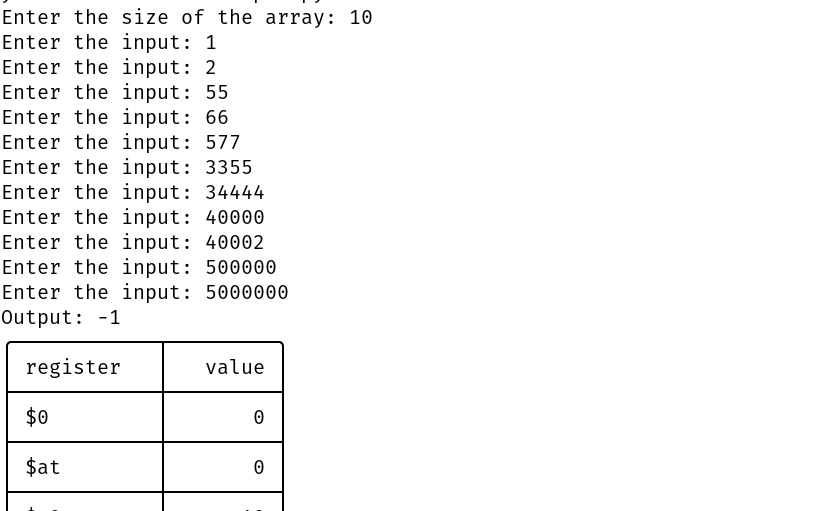
\includegraphics[width=1.0\textwidth]{CA/2-sum.jpeg}
    \caption{Result}
\end{figure}

\newpage

\begin{figure}[H] % Use the H placement option
    \centering
    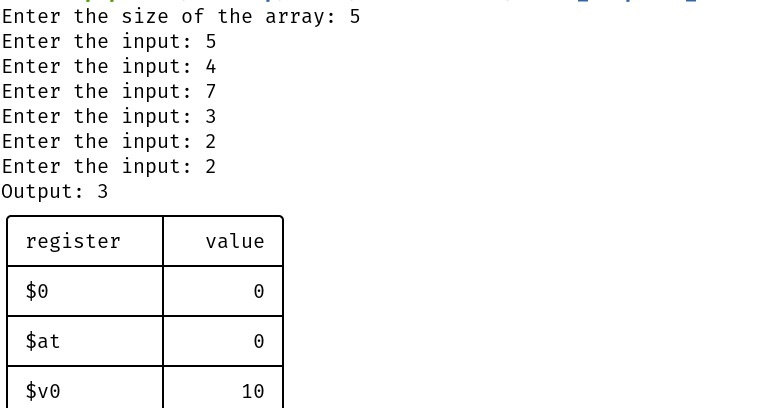
\includegraphics[width=1.0\textwidth]{CA/K-th smallest.jpeg}
    \caption{Result}
\end{figure}
\newpage

\begin{figure}[H] % Use the H placement option
    \centering
    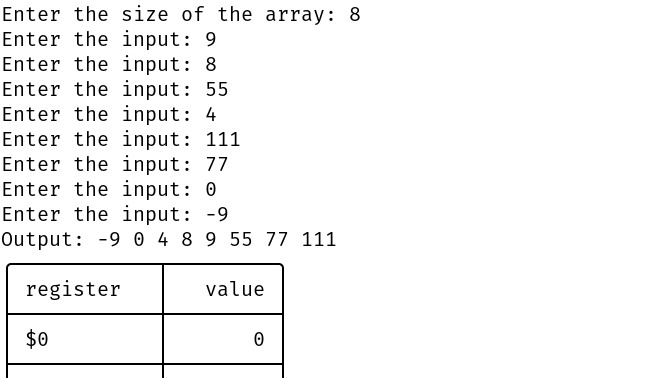
\includegraphics[width=1.0\textwidth]{CA/bubbleSort.jpeg}
    \caption{Result}
\end{figure}


\bibliographystyle{plain}
\bibliography{refs}

\end{document}